\section{Discussion of backgrounds}
\label{sec:bkgtypes}

As shown in Section~\ref{sec:yields}, the SM background to this study is dominated 
by \ttbar events. The contribution from single-top, diboson production ($WZ, ZZ$), 
is small. The diboson backgrounds will be estimated from Monte Carlo. 
The Monte Carlo acceptances for these processes will be corrected for differences between 
data and Monte Carlo lepton identification and trigger efficiencies, as determined using 
the tag-and-probe method.

We study the same sign dileptons for the \ttbar background based on their origin.
The dominant source of dileptons in \ttbar events are produced via, $t \rightarrow W b$; where 
$W \rightarrow \ell \nu $. We classify them as follows, based on truth matched to their ``parents'':

\begin{itemize}
\item Type-I: both leptons originate from real $W$ (including $W \rightarrow \tau \rightarrow \ell$) bosons, one with mis-reconstructed charge.
\item Type-II a): one of the leptons is from a real $W$ and the other originates from heavy flavor sources ($b, c$).
\item Type-II b): one of the leptons is from a $W$ and the other is a fake lepton.
\item Type-III: both leptons are fakes or from heavy flavor sources.
\end{itemize} 

\begin{figure}[htb]
\begin{center}
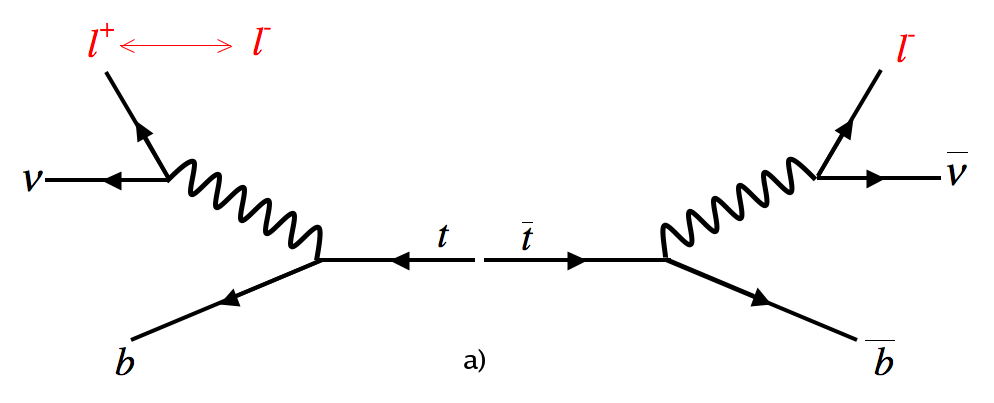
\includegraphics[width=0.32\linewidth, height=0.2\linewidth]{figs/feyntypeI.png}
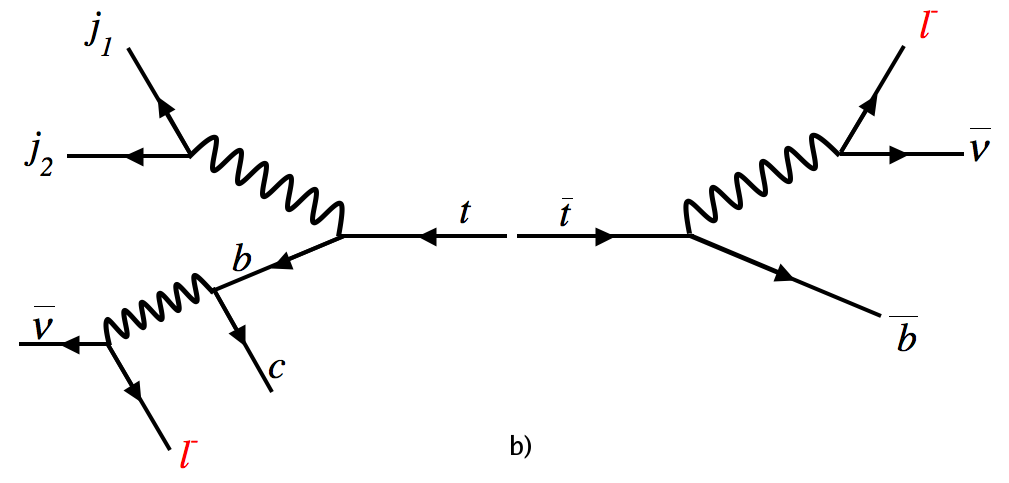
\includegraphics[width=0.32\linewidth, height=0.2\linewidth]{figs/feyntypeIIa.png}
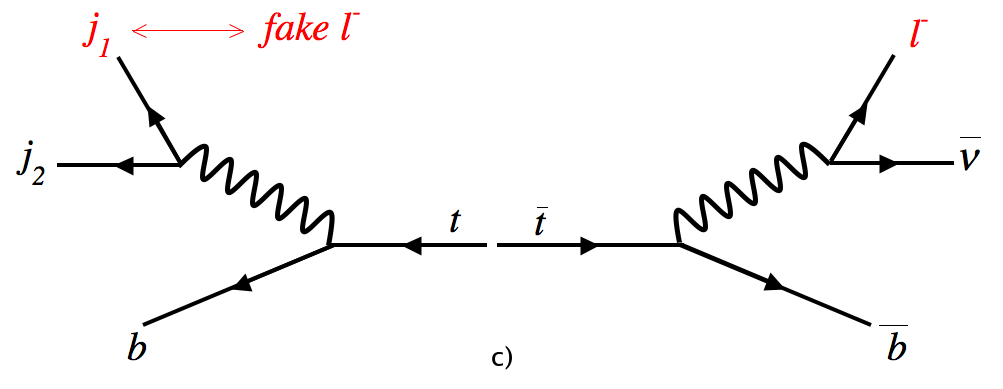
\includegraphics[width=0.32\linewidth, height=0.2\linewidth]{figs/feyntypeIIb.png}
\caption{ Classification of same sign dileptons from \ttbar decays. a) lepton from $W$ with mis-reconstructed charge; 
b) one of the lepton is from $W$, the other originating from heavy flavor sources; c) one of the lepton is from $W$,
and the other is a fake lepton. \label{fig:fakeOrigin}}
\end{center}
\end{figure}

Figure~\ref{fig:fakeOrigin} illustrates contribution from different types in \ttbar decays. The MC 
expectations of these contributions are given in Table~\ref{tab:fakeOrigin}.

\begin{table}[hbt]
\begin{center}
\begin{tabular}{|l|c|c|c|c|c|c|}\hline
Same Sign Leptons & Total & 	 Type-I &  Type-II & Type-II a) & Type-II b) & Type-III \\ \hline

$ee$ & 0.44$\pm$0.14 & 0.09$\pm$0.06 & 0.35$\pm$0.12 & 0.17$\pm$0.09 & 0.17$\pm$0.09 & 0.00$\pm$0.00 \\
$\mu\mu$ & 0.13$\pm$0.08 & 0.00$\pm$0.00 & 0.13$\pm$0.08 & 0.13$\pm$0.08 & 0.00$\pm$0.00 & 0.00$\pm$0.00 \\
$e\mu$ & 0.39$\pm$0.13 & 0.13$\pm$0.08 & 0.26$\pm$0.11 & 0.26$\pm$0.11 & 0.00$\pm$0.00 & 0.00$\pm$0.00 \\
total & 0.96$\pm$0.21 & 0.22$\pm$0.10 & 0.74$\pm$0.18 &	0.57$\pm$0.16 &	0.17$\pm$0.09 &	0.00$\pm$0.00 \\ \hline

\end{tabular}
\caption{ Expected number of \ttbar events of various types in 100 pb$^{-1}$ of integrated luminosity. Uncertainties are from MC statistics.\label{tab:fakeOrigin}}
\end{center}
\end{table}

It is interesting to note the following:
\begin{itemize}
\item Approximately $20 \%$, of the contribution is from Type-I (Charge mis-identification).
\item Almost all of the charge mis-identification is from electrons, in $ee$ and $e\mu$ channel.
\item The bulk of the \ttbar contribution in our event selection is from Type-II. The dominant among them 
is due to heavy flavor sources ($\sim 60 \%$).
\item No events with two fake leptons (Type-III) are expected within 100 pb$^{-1}$.
\end{itemize} 

In the following sections, we will briefly describe two different data driven approaches to 
estimate these contributions. The Type-I contribution will be estimated using the ``charge-flip rate'' described below, 
whereas the Type-II part will be estimated using the lepton fake rate method~\cite{fakelep}.



